%% Простая презентация с примером включения программного кода и
%% пошаговых спецэффектов
\documentclass{beamer}
\usepackage{fontspec}
\usepackage{minted}
\usepackage{xunicode}
\usepackage{xltxtra}
\usepackage{xecyr}
\usepackage{hyperref}
\usepackage{pgfplots}
\setbeamertemplate{footline}[frame number]
\setmainfont[Mapping=tex-text]{DejaVu Serif}
\setsansfont[Mapping=tex-text]{DejaVu Sans}
\setmonofont[Mapping=tex-text]{DejaVu Sans Mono}
\usepackage{polyglossia}
\setdefaultlanguage{russian}
\usepackage{graphicx}

\begin{document}
\title{Реализация библиотеки для потоковой записи файлов формата XLSX}
%%\subtitle{предварительные результаты}
\author{Свитков Сергей\\{\footnotesize\textcolor{gray}{группа 344\\научный руководитель: к.т.н, доц., Ю.В. Литвинов\\консультант: нач. отд. разр. ПО, "НТЦ Протей", М.В.\,Заведеев}}}
\institute{СПбГУ\\кафедра системного программирования}
\frame{\titlepage}

\begin{frame}\frametitle{Введение}
\begin{itemize}
    \item Веб-приложения в сфере биллинга, телекоммуникаций
    \item Различные отчеты, статистика
    \item Формат XLSX
    \item Потоковое формирование файла для экономии используемой RAM
\end{itemize}
\end{frame}

\begin{frame}\frametitle{Постановка задачи}
Цель: разработка библиотеки для потоковой записи файлов формата XLSX и сравнение её с существующими реализациями.
Для достижения этой цели были поставлены следующие задачи:
\begin{itemize}
    \item Сформулировать алгоритм, который будет использоваться для генерации файлов формата XLSX в потоковм режиме
    \item Реализовать предложенный алгоритм в виде переиспользуемой библиотеки с открытым исходным кодом, документацией, примерами использования и артефактом в Maven
    \item Сравнить полученную реализацию с существующими библиотеками по потреблению RAM (оперативной памяти) и скорости работы при создании документа
\end{itemize}
\end{frame}

\begin{frame}\frametitle{Обзор существующих решений}
\begin{itemize}
    \item Apache POI
    \begin{itemize}
        \item До версии 3.8 --- только in-memory
        \item Начиная с 3.8 --- Stream-API для записи, Event-API для чтения
        \item Часть операций всё равно только in-memory
        \item Отсутствие полных и подробных примеров работы с Stream-API
        \item Отсутствие поддержки автоматического разбиения документа на страницы
    \end{itemize}
    \item SJXLSX
    \begin{itemize}
        \item Не поддерживается с 2015 года
        \item Отсутствие документации
        \item Не поддерживается потоковая запись файлов
    \end{itemize}
\end{itemize}
\end{frame}

\begin{frame}\frametitle{Итоги обзора}
\begin{itemize}
    \item Apache POI поддерживает потоковую генерацию файлов, но всё же имеет ряд недостатков
    \item Реализовать свою библиотеку
    \item Сравнить её с рассмотренными реализациями
\end{itemize}
\end{frame}

\begin{frame}\frametitle{XLSX}
\begin{itemize}
    \item zip-архив с xml файлами
    \item Структура:
    \begin{itemize}
        \item \texttt{Content\_Types}.xml --- типы содержимого в архиве и пути к ним
        \item \texttt{\_rels} --- зависимости между файлами внутри архива
        \item docProps --- метаданные: имя автора, дата создания, ...
        \item xl --- директория с основными файлами архива: workbook, страницы, стили, таблицы
        \begin{itemize}
            \item Workbook --- метаданные, ссылки на страницы с данными
            \item Worksheets --- страницы с данными
        \end{itemize}
    \end{itemize}
\end{itemize}
\end{frame}

\begin{frame}\frametitle{Реализация: алгоритм}
\begin{itemize}
    \item Для каждой страницы создавать временный файл
    \item Хранить в RAM только один ряд (во время создания)
    \item После создания добавлять ряд во временный файл страницы
    \item После завершения формирования документа --- записывать данные из временных файлов в основной файл
    \item Для экономии дискового пространства сжимать временные файлы
\end{itemize}
\end{frame}

\begin{frame}\frametitle{Реализация: архитектура}
Упрощённая архитектура библиотеки:
\begin{figure*}
    \centering
    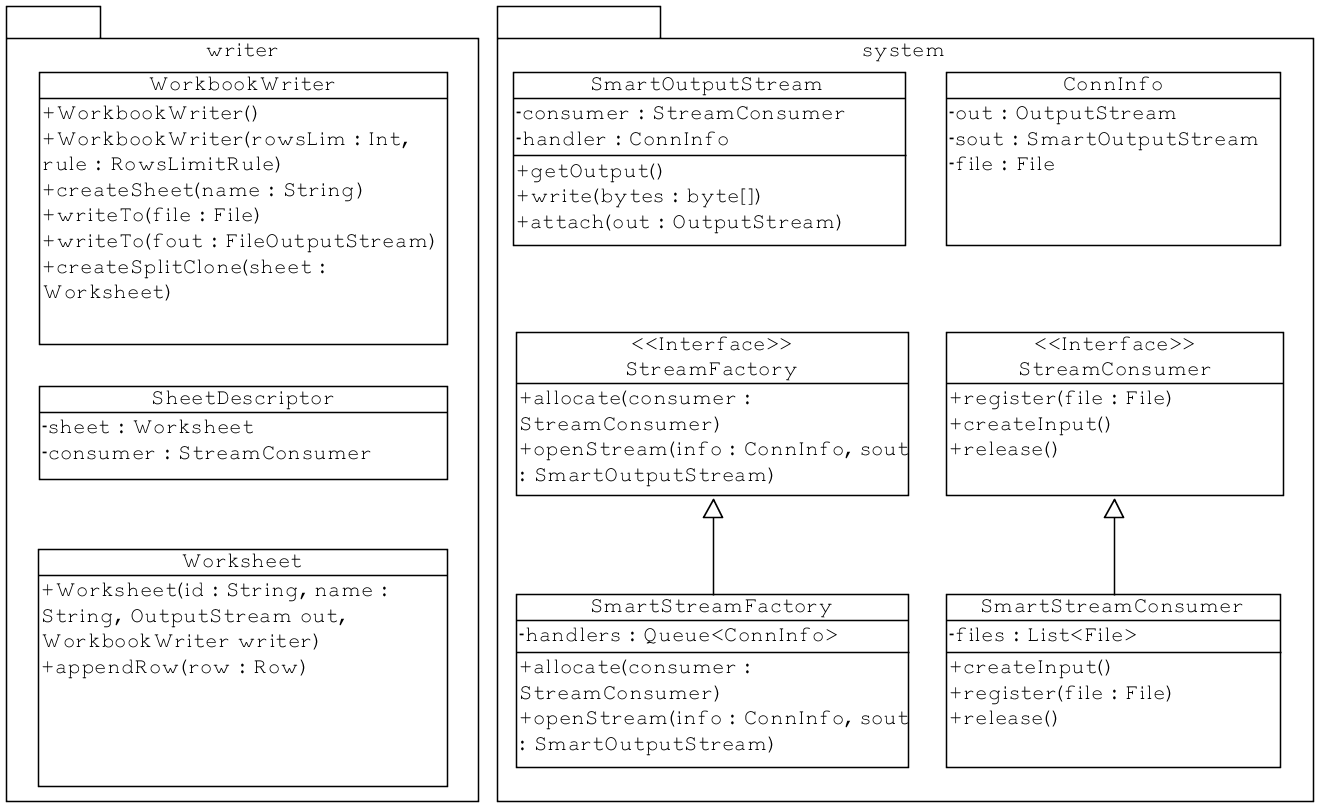
\includegraphics[height=7cm]{archsimple.png}
\end{figure*}
\end{frame}

\begin{frame}\frametitle{Эксперименты: RAM}
\begin{figure}[h]
    \centering    
    \def\svgwidth{\columnwidth}
    \input{tr.pdf_tex}
\end{figure}
\end{frame}

\begin{frame}\frametitle{Эксперименты: скорость записи}

\begin{figure}[h]
    \centering    
    \def\svgwidth{\columnwidth}
    \input{unt.pdf_tex}
\end{figure}
%\begin{figure*}
%    \centering
%     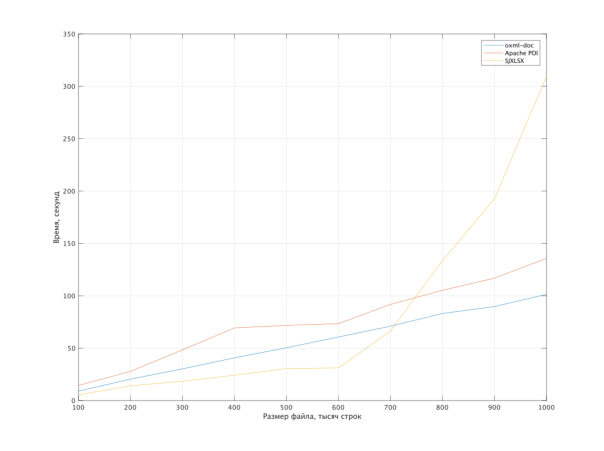
\includegraphics[width=\textwidth, keepaspectratio]{speed.pdf}
%\end{figure*}
\end{frame}

\begin{frame}\frametitle{Результаты}
В ходе данной работы были достигнуты следующие результаты:
\begin{itemize}
    \item Реализован предложенный в рамках работы алгоритм записи файлов формата XLSX
    \item Реализация оформлена в виде библиотеки для потоковой записи файлов формата XLSX с открытым исходным кодом и артефактов в Maven
    \item Проведено сравнение реализации с существующими библиотеками по количеству используемой RAM и скорости работы при создании документа
\end{itemize}
\end{frame}

%\lstset{language=java}
%\begin{frame}[fragile]\frametitle{Алгоритм}
%\begin{lstlisting}
%while (isWater()) {
%  row(boat);
%  if (crayfish) {
%    put(hand, river);
%  }
%}
%\end{lstlisting}
%\end{frame}

%\begin{frame}\frametitle{Результаты}
%\Large
%\begin{itemize}
%    \item Достигли
%    \begin{itemize}
%        \item того
%        \item сего
%    \end{itemize}
%    \item Получили
%    \item Обнаружили
%\end{itemize}
%\end{frame}
\end{document}